%   Copyright (C) 2014  School of Information Sciences, Manipal



\newcommand{\projecttitle}{Boot-Time Optimization for Android on Intel Atom Architecture}
\newcommand{\projectauthors}{\normalsize Aurabindo J}
\newcommand{\institutename}{School of Information Sciences}
\newcommand{\university}{Manipal University, Manipal}
\newcommand{\rollno}{141021001}
\documentclass{mainreport}
%\linespread{1.5}
\usepackage{hyperref}
\usepackage{makeidx}
\usepackage{multirow}
\usepackage{nomencl}
\usepackage{pdfpages}
\usepackage{subcaption}
\usepackage{tabularx}
\usepackage{listings}
\usepackage{color}
\usepackage{upquote}
%\usepackage{biblatex}

\definecolor{dkgreen}{rgb}{0,0.6,0}
\definecolor{gray}{rgb}{0.5,0.5,0.5}
\definecolor{mauve}{rgb}{0.58,0,0.82}


\lstset{frame=tb,
  aboveskip=3mm,
  belowskip=3mm,
  showstringspaces=false,
  columns=flexible,
  basicstyle={\small\ttfamily},
  numbers=none,
  numberstyle=\tiny\color{gray},
  keywordstyle=\color{blue},
  commentstyle=\color{dkgreen},
  stringstyle=\color{mauve},
  breaklines=true,
  breakatwhitespace=true
  tabsize=3
}

%\usepackage{tocloft}


\newcommand{\tab}{\hspace*{2em}}
% for removing dots

\makeatletter
\renewcommand{\@dotsep}{10000} 
\makeatother

\renewcommand{\figurename}{Fig.}


\begin{document}

\maketitle
\makecertificate

\parindent 10mm
%\newgeometry{bottom=2.5cm,top=2.5cm}
\chapter*{Acknowledgment}\label{ack}\addcontentsline{toc}{chapter}{Acknowledgment}
{\label{ack} 

%\paragraph*{•}
\hspace{6mm} This project itself is an acknowledgment to the inspiration, drive and technical
assistance contributed by many individuals. I would like to express my heartfelt thanks to my project guides 
{\bf Dr. Harishchandra Hebbar} and {\bf Dr. Nandish Rao}
%\paragraph*{•}
I would like to thank all the teaching and non teaching faculties of {\bf School of Information Sciences}, 
in particular, for providing us with an ample environment and
infrastructure required to carry out this project. 

This project would not be possible without the support from {\bf Intel India}. I thank \
{\bf Mr. Satish A Hipparagi}, Engineering Manager at Intel,
for the inspiration and support rendered.

%\paragraph*{•}
I extend my heartfelt thanks to my parents, friends and well wishers for their 
support and timely help. Above all I thank the Almighty for His blessing and 
providing mercies at all stages of my work. \\[2cm]




\noindent Manipal \hfill Project Members

\noindent \today \hfill \institutename

 \hfill Manipal





}

\chapter*{Abstract}\label{Abstract}\addcontentsline{toc}{chapter}{Abstract}

{
\label{Abstract}



%\paragraph*{•}
\hspace{6mm} Android was originally developed on ARM architecture in mind, and hence it is much more optimized on ARM rather than x86. The thesis aims at evaluating various known methods as well as finding new areas for optimization. Optimization effort will be targeting at reducing the boot time of the the system by evaluating various components which includes BIOS firmware, Bootloader, Linux Kernel and other AOSP components.
%\end{center}
}

%generate table of contents
\tableofcontents

%\chapter*{List of Symbols}\label{symbol}\addcontentsline{toc}{chapter}{List of Symbols}
%\listofsymbols

%\input{symbol}

%\input{fig}

\addcontentsline{toc}{chapter}{List of Figures}



\listoffigures
%\listoftables
\addtocontents{lof}{\textbf{No.}\hspace{8 mm}\textbf{Figure}~\hfill\textbf{Page}\par}
%\newpage


\chapter*{List of Abbreviations}\label{abbrv}\addcontentsline{toc}{chapter}{List of Abbreviations}




%Add your abbreviations here as follows
%\nomenclatue{Abbr}{Abbreviation}
%Example:
%\makenomenclature
\begin{center}
\label{abbrv}
\begin{tabular}{r l}
	TTYL & Talk To You Later \\
	AFAIK & As Far As I Know \\
	IMHO & In My Humble Opinion \\
	IMO & In My Opinion (not so humble)\\
	ROFL & Rolling On The Floor and Laughing
\end{tabular}
\end{center}


\newpage



%\chapter*{Report}\label{report}\addcontentsline{toc}{chapter}{Report}

\pagenumbering{arabic}





\section{Introduction}
\label{report}


\hspace{8mm} 

\noindent Mobile devices are the one of the most competitive consumer technology equipment market.
Manufacturers come up with improved or advanced versions of their product quite sooner that
people expect. With the demand from the market for more of performance, features, battery
life, etc the need to optimizing existing products also arise. Hence optimization of boot time
for Android devices are quite relevant.

We will look into the overview of Android booting sequence from all levels. Then we will look
deeply into available tools to evaluate the boot time. Various profiling tools which help understand
the booting process in detail will also be covered in detail. Finally we will look at the techniques
and procedures which will help in reducing the boot time. The optimizing effort will be focused on the
linux kernel and bootloader.

\subsection{About Android}

Android is an open source mobile OS currently developed by Google, based on the Linux kernel and designed
primarily for touchscreen mobile devices such as smartphones and tablets. Initially developed
by Android, Inc., which Google bought in 2005. Android was unveiled in 2007, along with the
founding of the Open Handset Alliance – a consortium of hardware, software, and telecommunication
companies devoted to advancing open standards for mobile devices. However, most Android devices
ultimately ship with a combination of open source and proprietary software, including proprietary
software required for accessing Google services.


Linux kernel is the core part of the Android OS. The version of the linux kernel used in Android is
based on one of the Linux kernel's LTS branches. Android's variant of the Linux kernel has further
architectural changes that are implemented by Google outside the typical Linux kernel development
cycle, such as the inclusion of components like Binder, ashmem, pmem, logger, wakelocks,
and different out-of-memory (OOM) handling.

\subsubsection {Hardware}

The main hardware platform for Android is the ARM architecture (ARMv7 and ARMv8-A architectures),
with x86 and MIPS architectures also officially supported in later versions of Android.
Since Android 5.0 "Lollipop", 64-bit variants of all platforms are supported in
addition to the 32-bit variants.

Intel has its processors specifically made for low power devices, which run Android.
This architecture is known as Intel Atom. It is a SoC which offers good performance with
reduced power consumption compared to a full fledged desktop processors known under
the series Intel Core.

\subsubsection{Software Stack}

On top of the Linux kernel, there are the middleware, libraries and APIs written in C,
and application software running on an application framework which includes
Java-compatible libraries based on Apache Harmony. Development of the Linux kernel
continues independently of other Android's source code bases.

\begin{figure}[h]
  \centering
    \centering
    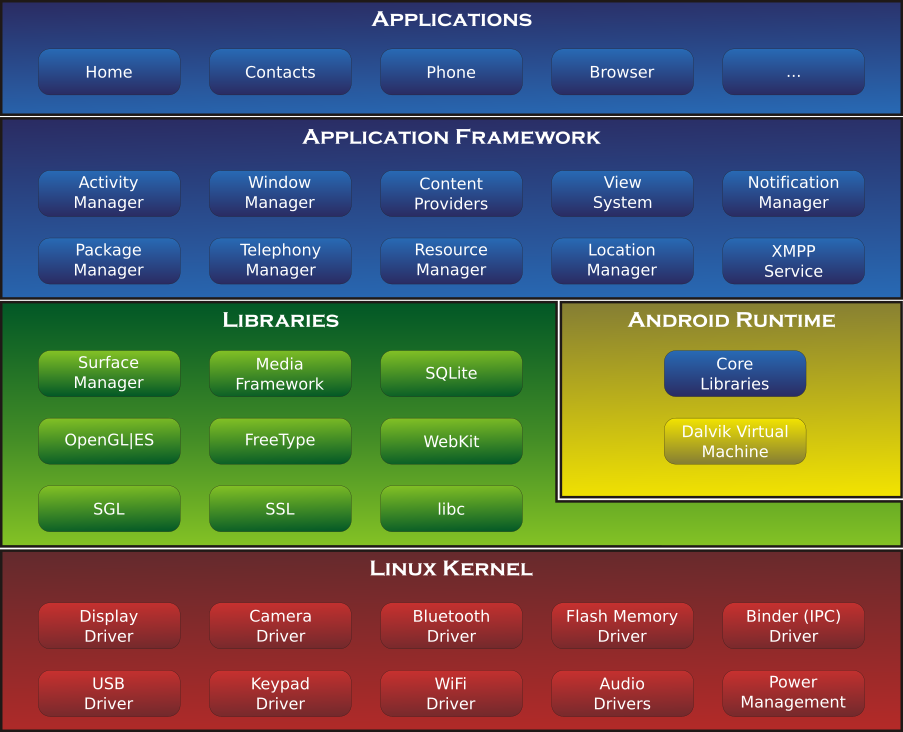
\includegraphics[scale=0.6]{android_arch.png}
    \caption{Android Software Architecture}
    \label{fig:android_arch}
\end{figure}

%\begin{figure}[h!]
%  \centering
%    	\includegraphics[scale=0.5]{scada_architecture.png}
%	\caption{Architecure of a typical power SCADA system}
%	\label{scada_arch} %the label was cycle here



%\begin{figure}[h]
%  \centering
%  \begin{subfigure}[b]{1\textwidth}
%    \centering
%    \includegraphics[scale=0.4]{digraph_simple.png}
%    \caption{relation digraph of the simplified system}
%    \label{fig:digraph_simple}
%  \end{subfigure}
  
%  \begin{subfigure}[b]{1\textwidth}
%    \centering
%    \includegraphics[scale=0.4]{digraph_virtual.png}
%    \caption{Representation of the digraph with virtual nodes}
%    \label{fig:digraph_virtual}
%  \end{subfigure}
  
%\end{figure}




\section{Android Boot Sequence}
\label{android_boot}


\hspace{8mm} 

\noindent At the core of Android is the Linux Kernel managing all the underlying hardware. Hence boot process is
similar to what we find in a Linux machine. However, the devices which run Android are highly
integrated devices, called SoCs, which have a wide range of devices which we dont find in
a normal linux desktop system or a laptop. Much of these devices come with proprietary drivers.
The bootloader usually used for ARM based SoCs, is called Uboot. However, for Intel Atom SoC
based on the Cherrytrail family uses a proprietary bootloader, called Kernelflinger.

Once Kernel is started, it does the driver initialization and call the first userspace program,
called init. From here, what init loads is making the difference as what we see Android as it is.

The diagram below shows the boot flow in Android:


\begin{figure}[h]
  \centering
    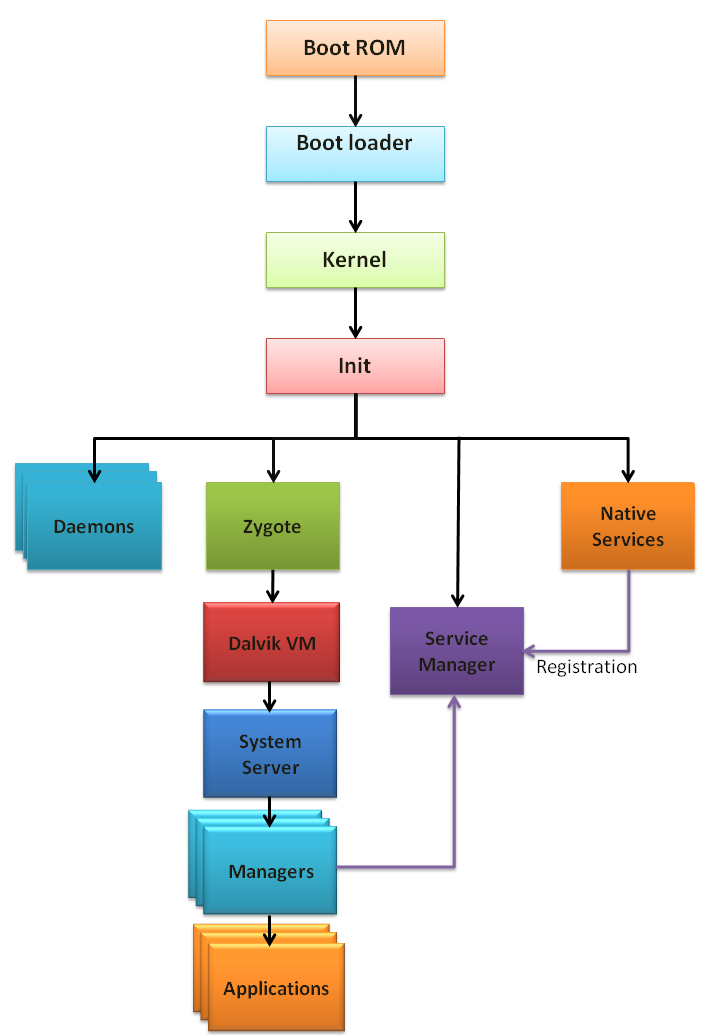
\includegraphics[scale=0.7]{android_boot.png}
    \caption{Android Boot Process}
    \label{fig:android_boot}
\end{figure}

\clearpage
\subsection{Bootloader}

Up on power up, the SoC firmware boots from a ROM area typically located internally,
different from the system's eMMC card. This is what we loosely call BIOS, for legacy
reasons. This code determines the boot media and loads the boot loader from the media.
The boot loader can be used to initialize the DRAM and load another level of loader
or directly the Linux kernel. On Cherrytrail Platform, the bootloader is called Kernelflinger.
It then loads the Linux Kernel with the required parameters hardcoded in the boot image.

\subsection{Kernel}

Linux kernel is the heart of the Android responsible for the process creation, inter process communication, device drivers, file system management etc. Android applies a custom patch on the main stream kernel to support certain features like Wake locks etc needed for operation of the Android.

The kernel is loaded as a compressed imaege. Up on loading, it decompresses itself,
does the driver initializations, mounts the root file system (typically passed 
as kernel command line arguments) and starts the first application in user space.


\subsection{Android}

Android typically operates wholly on the user space. The android applications are executed over a Virtual Machine called the Dalvik. The following section explains the internals in detail.

\subsubsection{init and init.rc}

The first user space application executed on booting the kernel is the init
executable located in the root folder. The process parses a start up script
called the \textit{init.rc} script. This is written in a language designed
for android used to start all the necessary processes, daemons and services
for a proper operation of android. It offers various types of execution timings
such as early-init, on-boot, on-post-fs etc. A detailed explanation of the
scripting model is available on Android documentation site.

\subsubsection{Demons and Services}

The init process creates various daemons and processes like rild, vold,
mediaserver, adb, etc each responsible for its own functionality.
Descriptions of these processes are not in the scope of this post.
Rather we will discuss more about \textit{Zygote} process.

\subsubsection{Service Manager}

The service manager process manages all the services running in the system.
Every service created registers itself with this process and this information
is used for future references by other processes/applications.

\subsubsection{Zygote}

Zygote is one of the first init process created on boot. The term ``zygote`` is based the biological ''initial cell formed
that divides to produce offsprings``. Similarly zygote in android initializes the Dalivik VM and
forks to create multiple instances to support each android process. It facilitates using a shared code
across the VM instances resulting in a low memory foot print and short load time, ideal for an embedded system.

Zygote apart from installing a listener on the server socket, also preloads classes and
resources to be used later in the Android applications. Once done, the system server is started.

%nbegin{figure}[h]
%  \centering
%  \begin{subfigure}[b]{1\textwidth}
%    \centering
%    \includegraphics[scale=0.4]{digraph_simple.png}
%    \caption{Relation digraph of the simplified system}
%    \label{fig:digraph_simple}
%  \end{subfigure}
  
%  \begin{subfigure}[b]{1\textwidth}
%    \centering
%    \includegraphics[scale=0.4]{digraph_virtual.png}
%    \caption{Representation of the digraph with virtual nodes}
%    \label{fig:digraph_virtual}
%  \end{subfigure}
  
%\end{figure}




%\chapter*{Datasheets}\label{datasheet}\addcontentsline{toc}{chapter}{Datasheets}

%{\label{nexys3}\includepdf[pages={-}]{Nexys3_rm.pdf} 
%{\label{nexys3}\includepdf[pages={1-1,8-10,11-14,18-20}]{Nexys3_rm.pdf} 
%{\label{nexys3}\includepdf[pages={1-1}]{spartan6.pdf} 

\nocite{*}
\bibliographystyle{plain}
\bibliography{master}

\end{document}
